\documentclass[twocolumn]{article}

\usepackage[utf8]{inputenc}
\usepackage[T1]{fontenc}
\usepackage{amsmath}
\usepackage{amsthm}
\usepackage{graphicx}
\usepackage{breqn}

\newcommand{\la}{\left\langle}
\newcommand{\ra}{\right\rangle}
\newcommand{\beq}{\begin{eqnarray}}
\newcommand{\eeq}{\end{eqnarray}}

\newcommand{\append}{\leftarrow{\mkern-18mu}{+}\:}

\newtheorem{lemma}{Lemma}
\newtheorem{theorem}{Theorem}

\title{DRAFT: A Family of Sparse, Vertex-Transitive Graphs}
\author{Edward L. Platt}
\date{August 2015}

\begin{document}

\maketitle

\section{Introduction}

\section{Network Structure}
\begin{figure}
\begin{center}
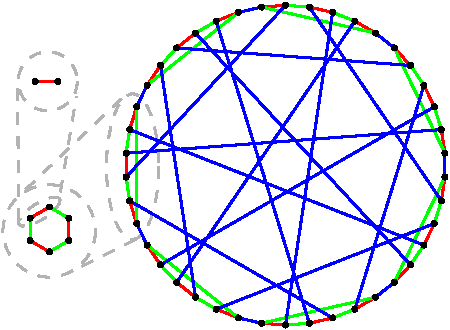
\includegraphics{g123}
\caption{
\label{fig:g123}
}
\end{center}
\end{figure}

\subsection{Partial network approximation}

\section{Construction}

We recursively construct a family of vertex-transitive graphs
$G_n = \la V_n, E_n \ra$.
The vertices $v \in V_n$ are labeled by an $n$-sequence of integers.
We define $G_0$ and $G_1$ as:
\beq
V_0 &=& \{ \la\ra \}, \\
E_0 &=& \{ \}, \\
V_1 &=& \{\la{0}\ra,\la{1}\ra\}, \\
E_1 &=& \left\{\{\la{0}\ra,\la{1}\ra\}\right\}.
\eeq
We construct subsequent vertex sets from copies of the previous set,
with each copy having a different integer appended to its vertex labels:
\beq
\label{eq:vn}
V_{n+1} &=& \bigcup_{k = 0}^{C_n}
\left\{ v | w \in V_n \land v = w \append k \right\},
\\
C_n &\equiv& |V_n|,
\eeq
where $w \append k$ denotes appending element $k$ to the end of sequence $w$.
We note that a one-to-one mapping $z_n$ exists between the vertices of $G_n$ and the
integers from $0$ to $C_n - 1$:
\beq
z_n(v) &=& \sum_{i=0}^{n-1} C_i v_i.
\eeq
We define even and odd subsets of $V_n$:
\beq
A_n &=& \{ v | v \in V_n \land v_0 = 1 \}, \\
B_n &=& \{ v | v \in V_n \land v_0 = 0 \}.
\eeq
We also define the following mappings on the vertices of $G_n$:
\beq
(\phi_k(v))_i
&=&
\begin{cases}
v_i + 1 \mbox{ mod } (C_i + 1) & \mbox{if } i = k,
\\
v_i & \mbox{otherwise},
\end{cases}
\\
(\psi_n(v))_i
&=&
\begin{cases}
v_i + 1 \mbox{ mod } (C_i + 1)
& \mbox{if } i = 0 \lor \forall j < i: v_j = C_j, \\
v_i & \mbox{otherwise},
\end{cases}
\\
\theta_n(v)
&=&
\begin{cases}
\psi_n(v) & \mbox{if } v \in A_n, \\
\psi_n^{-1}(v) & \mbox{if } v \in B_n,
\end{cases}
\eeq
with $i, k < n$.

To construct the edges of $G_{n+1}$ we define a ``shortcut'' function $s_n(j, k)$
with $j \in \{0, 1, C_n - 1\}$ and $k \in \{0, 1, 2, \ldots, C_n\}$ which
determines the interconnections between copies of $G_n$.
\beq
\label{eq:shortcut}
s_{n}(j, k)
&=&
\begin{cases}
k + 1 \ \mbox{mod } (C_n + 1)
&
\mbox{if } j = C_n - 1,
\\
k - 1 \ \mbox{mod } (C_n + 1)
&
\mbox{if } j = 0,
\\
k + j + 1 \ \mbox{mod } (C_n + 1)
&
\mbox{if } j \in \{1, 3, \ldots, C_n - 3\},
\\
k - j \ \mbox{mod } (C_n + 1)
&
\mbox{if } j \in \{2, 4, \ldots, C_n - 2\}.
\end{cases}
\eeq
We also define a parity selector function on the edges $e \in E_n$:
\beq
p_x(e)
&=&
v \quad \mbox{s.t. } v \in e \land v_0 = x.
\eeq
The edges of $G_{n+1}$ are then given by:
\beq
\label{eq:edgesrecursive}
R_{n+1}
&=&
\bigcup_{k=0}^{C_n}
\bigcup_{e \in E_n} \{ p_0(e) \append k, p_1(e) \append k\},
\\
\label{eq:edgesshortcut}
S_{n+1}
&=&
\bigcup_{k=0}^{C_n}
\bigcup_{v \in A_n} \{ v \append k, \theta_n(v) \append s_n(z_n(v), k) \},
\\
&=&
\bigcup_{k=0}^{C_n}
\bigcup_{v \in B_n} \{ v \append k, \theta_n(v) \append s_n(z_n(v), k) \},
\\
E_{n+1}
&=&
R_{n+1} \cup S_{n+1},
\eeq
noting that $S_{n+1}$ can be written in terms of either the odd vertices $A_n$
or the even vertices $B_n$.
Eq. (\ref{eq:edgesrecursive}) replicates the edges of
$G_n$ among subsets of the vertices of $G_{n+1}$,
while Eq. (\ref{eq:edgesshortcut})
creates one edge between each pair of the subsets.

\section{Properties of $G_n$}

\begin{lemma}
\label{lem:regular}
The graph $G_n$ is $n$-regular for all $n \geq 0$.
\end{lemma}
\begin{proof}
We proceed using induction on $n$.
The base case $G_1$ is $1$-regular by inspection.
In the inductive case $G_{n+1}$,
Eq. (\ref{eq:edgesrecursive})
reproduces the edges of $G_n$,
which is $n$-regular by induction,
contributing $n$ to the degree of each vertex.
Eq. (\ref{eq:edgesshortcut}) adds one to the degree of each odd vertex.
As $\theta_n$ is a bijective map between odd and even vertices,
Eq. (\ref{eq:edgesshortcut}) also adds one to the degree of each even vertex,
giving a total degree of $n + 1$.
\end{proof}

\begin{lemma}
The number of vertices and edges of the graph $G_n$ are given by the recurrence
relations:
\beq
C_0 = |V_0| &=& 1, \\
\label{eq:cnrec}C_{n} = |V_{n}| &=& C_{n-1} (C_{n-1} + 1), \\
|E_n| &=& \frac{n}{2} C_n.
\eeq
\end{lemma}
\begin{proof}
The vertex set of $G_n$, given by Eq. (\ref{eq:vn}), is a union of
$C_{n-1} + 1$ sets.
The vertex labels within each set all end with the same element,
and this element is unique to each set.
The sets are thus disjoint.
Each set contains $C_{n-1}$ elements, giving $C_{n-1}(C_{n-1} + 1)$
elements.
By Lemma \ref{lem:regular}, $G_n$ is $n$-regular and has
$\frac{n}{2}|V_n| = \frac{n}{2}C_n$ edges.
\end{proof}
\begin{lemma}
\label{lem:phiauto}
The mapping $\phi_{n-1}$ is an automorphism of $G_n$.
\end{lemma}
\begin{proof}
Let $v$ be a vertex in $V_n$.
$\phi_{n-1}$ has no effect on $v_0^{n-2}$ so it preserves the edges $R_n$,
defined in Eq. (\ref{eq:edgesrecursive}).
The vertex $v$ has exactly one other edge, from $S_n$ defined in
Eq. (\ref{eq:edgesshortcut}):
\beq
e &=& \{ v, \theta_n(v_0^{n-2} \append s_n(z_n(v_0^{n-2}), v_{n-1}) \}.
\eeq
Applying $\phi_{n-1}$ to both vertices gives:
\beq
\tilde{e} &=&
\{ v_0^{n-2} \append (v_{n-1} + 1) \mbox{ mod } (C_{n-2} + 1), \\
&& \quad \theta_n(v_0^{n-2} \append
s_n(z_n(v_0^{n-2}), (v_{n-1} + 1) \mbox{ mod } (C_{n-2} + 1) ) \},
\\
&=&
\{ v_0^{n-2} \append \tilde{k},
\theta_n(v_0^{n-2} \append s_n(z_n(v_0^{n-2}), \tilde{k}) \},
\eeq
where $\tilde{k} = (v_{n-1} + 1) \mbox{ mod } (C_{n-2} + 1)$.
The edge $\tilde{e}$ is also a member of $S_n$,
showing that $\phi_{n-1}$ permutes the elements of $S_n$,
and preserves all edges in $E_n$.
\end{proof}
\begin{theorem}
The graphs $G_n$ are vertex-transitive for all $n \geq 0$.
\end{theorem}
\begin{proof}
The graph $G_0$ is trivially vertex-transitive.
For higher order graphs,
we recursively construct a mapping $\Phi_n$
that maps an arbitrary vertex $v \in V_n$ to
an arbitrary vertex $\tilde{v} \in V_n$ and preserves the edges in $E_n$.
Let $\delta_i = \tilde{v}_i - v_i \mbox{ mod } (C_i + 1)$.
For the subsequence $v_0^0$, the map $\Phi_1 = \phi_0^{\delta_0}$
achieves the desired mapping and preserves the edges in $E_1$ by
Lemma \ref{lem:phiauto}.
Given an edge-preserving mapping $\Phi_n$
from $v_0^{n-1}$ to $\tilde{v}_0^{n-1}$,
we can construct $\tau_{n}$.
We define mappings $\pi_n$ and $\tau_{n}$:
\beq
\pi_n(0) &=& 0
\\
\pi_n(s_n(v_0^{n-1}, 0))
&=& s_n(\Phi_n(v_0^{n-1}), 0)
\\
\tau_{n}(v)
&=& \Phi_{n}(v_0^{n-1}) \append \pi_n(v_n).
\eeq
For the recursive edges defined in Eq. (\ref{eq:edgesrecursive})
$\{v_0^n, w_0^n\} \in R_{n+1}$:
\beq
\{ \tau_{n}(v_0^n), \tau_{n}(v_0^n)
&=&
\{ \Phi_n(v_0^n) \append \pi_n(k), \Phi_n(w_0^n) \append \pi_n(k)\}
\\ &=&
\{ \tilde{v}_0^n \append \tilde{k}, \Phi_n(\tilde{w}_0^n) \append \tilde{k}\},
\eeq
which is simply another member of $R_{n+1}$.
As $\tau_{n}$ is bijective, it permutes the edges of $R_{n+1}$.
For the shortcut edges defined in Eq. (\ref{eq:edgesshortcut})
$\{v_0^n, w_0^n\} \in S_{n+1}$, when $v_n=0$:
\beq
\{\tau_{n}(v_0^n), \tau_{n}(w_0^n)\}
&=&
\{ \Phi_n(v_0^n) \append \pi_n(0),
\\ &&
\quad \Phi_n(w_0^n)) \append \pi_n(s_n(z_n(v_0^n), 0)) \}
\\ &=&
\{ \tilde{v}_0^n \append 0,
\tilde{w}_0^n \append s_n(z_n(\Phi_n(v_0^n)), 0) \}
\\ &=&
\{ \tilde{v}_0^n \append 0,
\theta_n(\tilde{v}_0^n) \append s_n(z_n(\tilde{v_0^n}), 0) \},
\eeq
showing that $\tau_{n}$ permutes the subset of edges in $S_{n+1}$ for which
$v_n=0$.
Consequently, because $\phi_n$ is an automorphism of $G_{n+1}$
by Lemma \ref{lem:phiauto}, $\tau_{n}$ also permutes the edges of the
subsets for which $(\phi_n^{-k}(v_0^n))_n=0$.
Those edges are the subset of $S_{n+1}$ for which $v_n=k$,
showing that $\Phi_n{n+1}$ permutes all edges within $S_{n+1}$ and
$E_{n+1}$.
We finish by applying the automorphism $\phi_n^{\delta_n}$:
\beq
\Phi_{n+1}(v) &=& \phi_n^{\delta_n}(\tau_{n}(v)),
\eeq
completing the mapping from $\tilde{v}$ to $\tilde{w}$.
\end{proof}
\section{Acknowledgements}
% Tony Garnock-Jones
% Cesar Hidalgo
% Grant Schoenebeck
% Aram Harrow
% Joe Nievelt
\section{To Do}
\begin{enumerate}
\item{Change Eq. (\ref{eq:shortcut}) to $C_n - j + k \ (\mbox{mod } C_n + 1)$ to reduce cases.}
\item{Prove degree as function of $n$ following \cite{aho1973}.}
\end{enumerate}
\bibliographystyle{plain}
\bibliography{vtgraph}

\end{document}
